\chapter{Architecture}
\label{cha:architecture}

This chapter is dedicated to displaying and describing the numerous components,
their relationships, and the general needs for the cluster architecture's composition.
\\ %
Understanding how the cluster works lays a good foundation for the following chapters,
in which almost everything seen here is extensively explained in terms of how it
was developed and why certain decisions were taken. Furthermore, the design is
dynamic and may be modified to include more or fewer components and/or
requirements to better meet the requirements of the end user. \\ %
Section \ref{subsec:architecture_cluster_example} depicts a real-world
functioning example of the cluster design given. \\ %
It has been extensively tested and is continuously operational 24 hours a day, hosting
a variety of services. Furthermore, it upscales or downscales automatically dependent
on demand or requirements. \\ %
The diagram below depicts an overview of the architecture, encompassing its
components and how they are interconnected, as well as a potential connection to
an external network.

\begin{figure}[htbp]
  \centering
  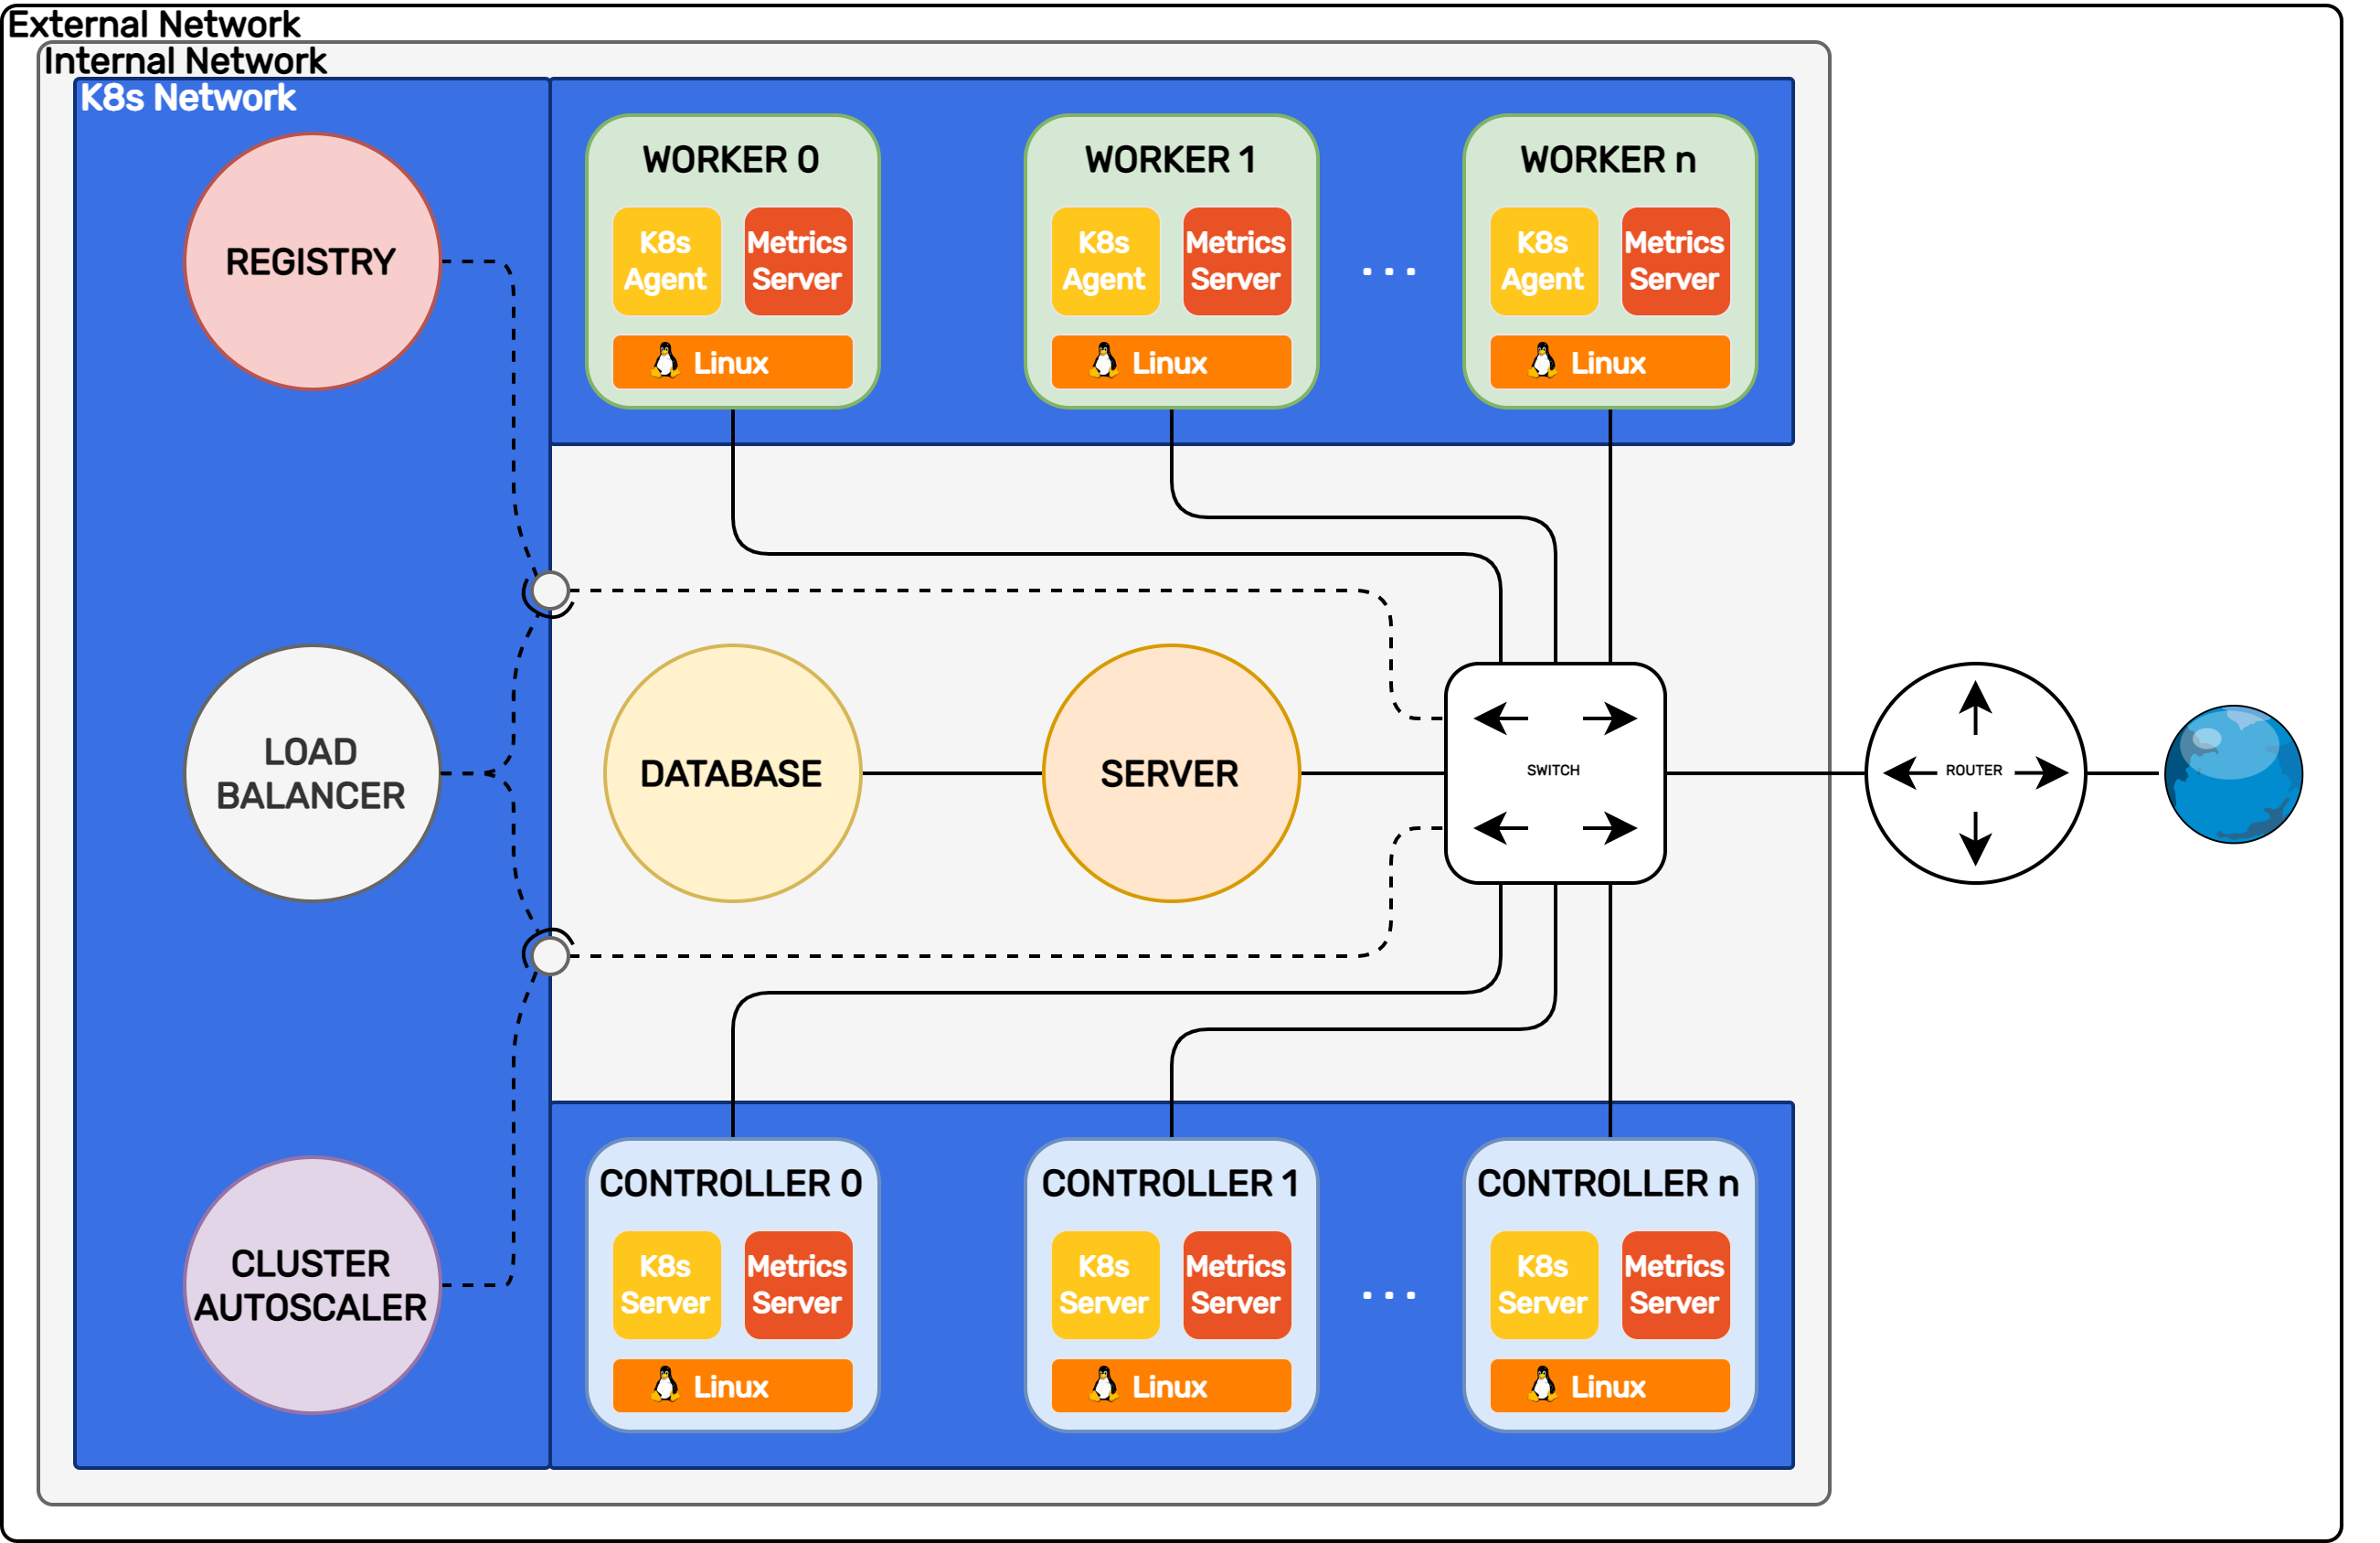
\includegraphics[width=\textwidth]{images/recluster/architecture.png}
  \caption{Architecture overview}
\end{figure}

\section{Components}
\label{sec:architecture_components}

\subsection{Controller}
\label{subsec:architecture_components_controller}

\subsection{Worker}
\label{subsec:architecture_components_worker}

\subsection{Server}
\label{subsec:architecture_components_server}

\subsection{Database}
\label{subsec:architecture_components_database}

\subsection{Registry}
\label{subsec:architecture_components_registry}

\subsection{Cluster Autoscaler}
\label{subsec:architecture_components_cluster_autoscaler}

\section{Network}
\label{sec:architecture_network}

\subsection{Domain}
\label{subsec:architecture_network_domain}

\section{Cluster}
\label{sec:architecture_cluster}

\begin{wrapfigure}
  {r}{.5\textwidth}
  \centering
  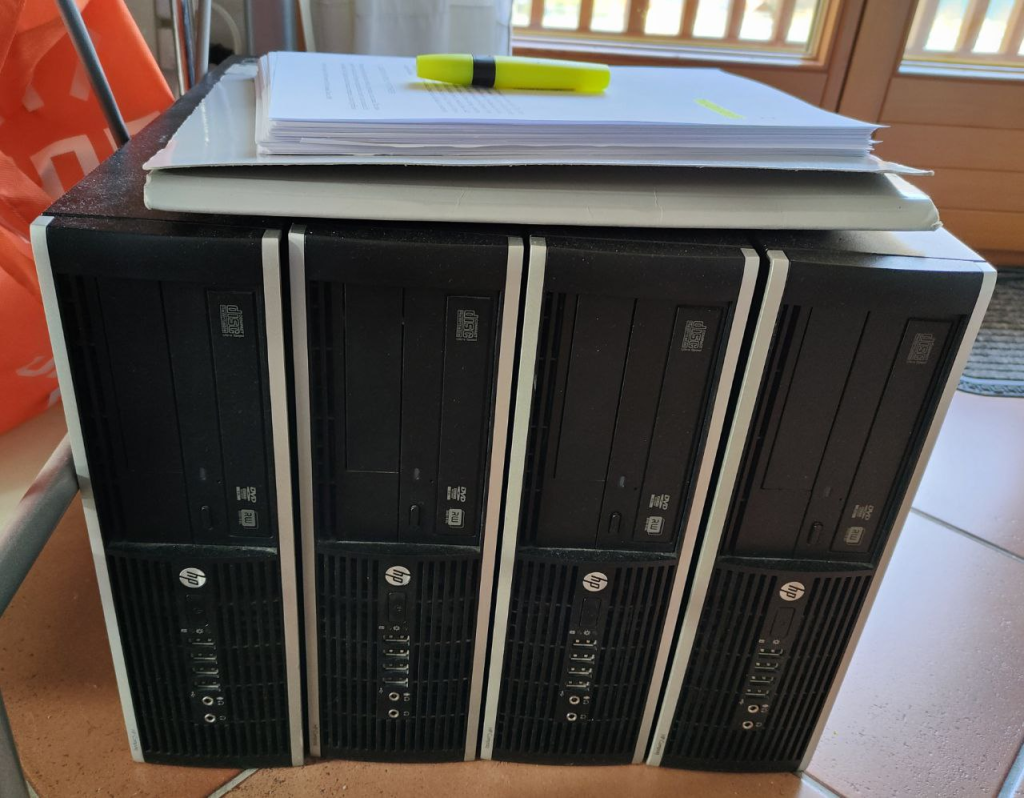
\includegraphics[width=.5\textwidth]{images/recluster/cluster.png}
  \caption{reCluster cluster}
\end{wrapfigure}

\subsection{Hardware}
\label{subsec:architecture_cluster_hardware}

% TODO WoL features, how to turn on nodes
% TODO Prefer nodes with WoL upscaling

\subsection{Example}
\label{subsec:architecture_cluster_example}

% TODO Move